\section{一般の $X_d$ に存在する trivial-normal symplectic curve}
\label{tnc:section}

第\ref{fnc:section}節の障害は、generic plane section の normal degree が $2d$ であることに由来する。
一方、normal degree が零となる別の symplectic curve を選べば、
第\ref{fhr:section}節の focus--hyperbolic block を閉曲線全体に適用できる。
本節では、そのような曲線が任意の smooth $X_d$ と所定の K\"ahler form に対して存在することを示す。
曲線は special algebraic hypersurface 上で作り、symplectic deformation によって所定の $X_d$ へ移す。
移送後の曲線が、所定の complex structure に関して holomorphic であるとは主張しない。

\subsection{Plane curve を含む smooth hypersurface の構成}

\begin{lemma}[Degree $d-2$ の plane curve を含む smooth member]\label{tnc:special-member}
$d\ge6$、$e=d-2$ とする。
Smooth plane curve $C_e\subset\mathbb P^2\subset\mathbb P^4$ と、
それを含む smooth degree-$d$ hypersurface $Y_d$ を選べる。
このとき
\begin{equation}\label{tnc:algebraic-data}
 \deg C_e=e,\qquad
 g(C_e)=\frac{(e-1)(e-2)}2,\qquad
 \det N_{C_e/Y_d}\simeq\mathcal O_{C_e}.
\end{equation}
\end{lemma}

\begin{proof}
Plane を $z_3=z_4=0$ とし、その上の任意の smooth degree-$e$ polynomial
$q_e(z_0,z_1,z_2)$ を取る。例えば Fermat polynomial が使える。
$C_e=\{z_3=z_4=q_e=0\}$ は complete intersection of degrees $(1,1,e)$ である。
Degree-$d$ polynomials の vector space
\[
 V=q_e H^0(\mathbb P^4,\mathcal O(2))
   +z_3 H^0(\mathbb P^4,\mathcal O(d-1))
   +z_4 H^0(\mathbb P^4,\mathcal O(d-1))
\]
を考える。その base locus はちょうど $C_e$ である。
以下、general $F\in V$ の hypersurface が全点で smooth となることを、first jets から確認する。

$p\notin C_e$ では、$q_e,z_3,z_4$ の少なくとも一つが非零である。
対応する coefficient の degree は $2$ または $d-1$ で、いずれも正である。
Projective space 上の $\mathcal O(m)$、$m\ge1$ の global sections は任意の点で
value と四つの first derivatives を独立に指定できる。
非消失 generator の乗法は first-jet space 上で可逆なので、
\[
 V\longrightarrow J_p^1\mathcal O(d)
\]
は全射である。従って $F=0$ が $p$ で singular となる条件は $V$ における五つの独立な linear conditions である。
$N=\dim\mathbb P(V)$ とすれば、$p\notin C_e$ にわたる singular-member incidence の次元は高々
$N-5+4=N-1$ である。

$p\in C_e$ では $F(p)=0$ と tangent derivative の消失は自動的である。
Normal derivatives の基底は $dq_e,dz_3,dz_4$ であり、
\[
 F=q_eR_2+z_3G_{d-1}+z_4H_{d-1}
\]
における三つの値 $R_2(p),G_{d-1}(p),H_{d-1}(p)$ は独立に指定できる。
従って singular 条件の codimension は三で、$C_e$ 上の incidence の次元は高々
$N-3+1=N-2$ である。
Singular pairs の全 incidence は $\mathbb P(V)\times\mathbb P^4$ 内で closed であり、
projective projection により singular members の集合も closed である。
上の次元評価からそれは proper subset なので、その外の $F$ を選べば $Y_d=\{F=0\}$ は smooth である。
これはこの linear system に対する Bertini smoothness の直接的な first-jet 証明である。

Plane curve の adjunction により $K_{C_e}\simeq\mathcal O_{C_e}(e-3)$ なので、genus formula を得る。
また smooth inclusions の normal exact sequence は
\[
 0\longrightarrow N_{C_e/Y_d}
 \longrightarrow
 \mathcal O_{C_e}(e)\oplus\mathcal O_{C_e}(1)\oplus\mathcal O_{C_e}(1)
 \longrightarrow\mathcal O_{C_e}(d)\longrightarrow0.
\]
最後の arrow が全射なのは $Y_d$ が $C_e$ に沿って smooth であるためである。
Determinant を取ると
\[
 \det N_{C_e/Y_d}
 \simeq\mathcal O_{C_e}(e+2-d)
 =\mathcal O_{C_e},
\]
となる。
\end{proof}

\subsection{所定の hypersurface と K\"ahler form への移送}

\begin{lemma}[Smooth hypersurfaces 間の symplectic 移送]\label{tnc:transport}
任意の二つの smooth degree-$d$ hypersurfaces $Y_d,X_d\subset\mathbb P^4$ は、
restricted Fubini--Study forms に関して symplectomorphic であり、その symplectomorphism は
hyperplane cohomology class を保つよう選べる。
さらに $[\omega]=\mathfrak a\mathsf H$ を満たす所定の K\"ahler form $\omega$ に対して
\[
 (Y_d,\mathfrak a\omega_{\rm FS}|_{Y_d})
 \simeq (X_d,\omega)
\]
という symplectomorphism が存在する。
ここでは $[\omega_{\rm FS}]=\mathsf H$ と規格化する。
\end{lemma}

\begin{proof}
Degree-$d$ hypersurfaces の projective parameter space における discriminant は proper algebraic subset である。
二つの smooth members を結ぶ projective line は discriminant に含まれず、その交わりは有限集合である。
従ってその有限集合を避ける smooth path を選べる。
Path 上の universal hypersurface family $\mathcal X_I\to[0,1]$ は proper smooth submersion である。
任意の horizontal lift of $\partial_t$ を取り、compactness を使って流せば、
smooth identifications $\psi_t:Y_d\to X_t$ を得る。
これはこの場合の Ehresmann trivialization の直接の flow construction である。

Restricted Fubini--Study forms の pullback
$\omega_t=\psi_t^*(\omega_{\rm FS}|_{X_t})$ は symplectic forms の smooth path である。
Ambient Fubini--Study form は closed なので、Cartan formula により
\[
 \frac{d}{dt}\omega_t=d\beta_t
\]
となる smooth one-forms $\beta_t$ がある。
同じ事実は、ambient hyperplane class が whole family 上で定まることからも分かる。
従って Moser theorem を $Y_d$ 上で適用すると、
$h_t^*\omega_t=\omega_0$ となる isotopy $h_t$ を得る。
$\psi_1\circ h_1$ が最初の symplectomorphism である。
Hyperplane class は family に沿って保たれ、Moser isotopy もその class を変えない。

次に所定の $X_d$ 上で
\[
 \omega_t'=(1-t)\mathfrak a\omega_{\rm FS}|_{X_d}+t\omega
\]
を取る。両端は同じ complex structure の K\"ahler forms なので、全ての $\omega_t'$ が K\"ahler である。
また cohomology class は一定である。
再び Moser theorem を適用し、最初の symplectomorphism と合成すれば結論を得る。
用いた Moser argument は \cite[Section 7.2]{cds-local} の標準的なものと同じである。
\end{proof}

\begin{theorem}[任意の $X_d$ における closed trivial-normal curve]\label{tnc:actual-curve}
$d\ge6$、$X_d\subset\mathbb P^4$ を任意の smooth hypersurface、
$\omega$ を所定の K\"ahler form、$[\omega]=\mathfrak a\mathsf H$ とする。
このとき $(X_d,\omega)$ 内に closed embedded symplectic surface $C'$ が存在し、
\begin{equation}\label{tnc:actual-data}
 \begin{split}
 \langle\mathsf H,[C']\rangle&=d-2,\qquad
 \operatorname{Area}_\omega(C')=(d-2)\mathfrak a,\\
 g(C')&=\frac{(d-3)(d-4)}2,\qquad
 N_{C'/X_d}\simeq C'\times\mathbb R^4
 \quad\text{as symplectic bundles}.
 \end{split}
\end{equation}
特に $C'$ 全体に沿う actual product neighborhood が存在する。
\end{theorem}

\begin{proof}
補題\ref{tnc:special-member}の pair $(Y_d,C_e)$、$e=d-2$ を取り、
補題\ref{tnc:transport}の symplectomorphism で $C_e$ を $C'$ へ移す。
Genus、hyperplane degree、面積は式\eqref{tnc:actual-data}の通りである。
Symplectomorphism は symplectic normal bundles を同型に移す。
Complex curve $C_e\subset Y_d$ の symplectic normal bundle の $c_1$ は、その holomorphic normal bundle の $c_1$ と一致する。
補題\ref{tnc:special-member}によりそれは零である。

Closed surface 上の complex rank-two bundle は $c_1=0$ なら smooth に自明である。
これは定理\ref{fnc:surface-criterion}の十分性の証明で示した unit section と complement line の議論である。
Unitary frame を取れば symplectic trivialization となる。
最後に補題\ref{fhr:product-neighborhood}を $r=0$ で適用する。
ここでは holomorphic normal bundle 自体の holomorphic triviality は必要なく、また主張していない。
\end{proof}

\paragraph{曲線を選ぶための数値条件.}
任意の closed embedded symplectic surface $S\subset X_d$ について、
$e=\langle\mathsf H,[S]\rangle$ とすれば tangent--normal splitting から
\begin{equation}\label{tnc:adjunction-balance}
 \langle c_1(N_{S/X_d}),[S]\rangle
 =(5-d)e-(2-2g(S))=2g(S)-2-(d-5)e.
\end{equation}
従って閉曲線全体で normal focus Cartan を保つための線形条件は
$2g(S)-2=(d-5)e$ である。今回の $e=d-2$ の曲線はこれを満たす。
この等式だけから曲線の存在を推論したのではなく、前の二補題で実際に構成した。

\begin{corollary}[Trivial-normal 曲線の次数と焦点ブロック数の数値制約]
\label{tnc:degree-genus-parity}
$d\ge6$ とし，$X_d\subset\mathbb P^4$ を smooth degree-$d$ hypersurface，
$S\subset X_d$ を connected closed embedded symplectic surface とする．
$e=\langle\mathsf H,[S]\rangle>0$，$g=g(S)$ とおく．
Symplectic normal bundle $N_{S/X_d}$ が自明なら
\[
 2g-2=(d-5)e.
\]
従って $d$ が偶数の場合には $e$ は偶数である．
さらに，$S$ に極大・極小のない circle-valued Morse map を選び，
その Reeb graph が一価頂点のない三価graphであるなら，
graphの頂点数，従って曲線方向の saddle の数は
\[
 n=2g-2=(d-5)e
\]
に限られる．この制約は埋め込みの実現可能性を十分に特徴付けるものではない．
\end{corollary}

\begin{proof}
Adjunction は
$c_1(TX_d)=(5-d)\mathsf H$ を与える．
Symplectic bundle の分解 $TX_d|_S=TS\oplus N_{S/X_d}$ から
\[
 0=\langle c_1(N_{S/X_d}),[S]\rangle
  =(5-d)e-(2-2g)
\]
となる．$2g-2$ は偶数なので $d-5$ が奇数なら $e$ は偶数である．
最後に，closed surface上のMorse関数のEuler公式は，
極大・極小がなくsaddleだけなら
$\chi(S)=-n$ を与える．三価graphの頂点はこれらのsaddlesに対応する．
\end{proof}

\subsection{曲線方向の自由端を持たない actual focus--hyperbolic block}

\begin{corollary}[Closed curve 上の non-elliptic block]\label{tnc:closed-block}
定理\ref{tnc:actual-curve}の $C'\subset(X_d,\omega)$ に対し、
$C'$ 全体とその十分小さい full normal neighborhood を含む compact domain with corners
$\mathcal U\subset X_d$ と、connected Lagrangian fibers を持つ quotient
\[
 \Pi:\mathcal U\longrightarrow R\times\Gamma
\]
が存在する。$R$ は補題\ref{fhr:focus-block}の compact rectangle、
$\Gamma$ は一価頂点のない finite trivalent graph である。
$n=(d-2)(d-5)$ と置けば
\begin{equation}\label{tnc:block-counts}
 \#V(\Gamma)=n,\qquad \#E(\Gamma)=\frac{3n}{2},\qquad
 b_1(\Gamma)=\frac{(d-3)(d-4)}2,
 \qquad \chi(\mathcal U)=-n.
\end{equation}
Regular fibers は $T^3$ である。
各 vertex $v$ と normal focus value $o\in\operatorname{int}R$ の組 $(o,v)$ 上には、
whole fiber $\mathcal N\times(S^1\vee S^1)$ があり、Euler 数は $-1$、
唯一の rank-zero point の Williamson type は $(0,1,1)$ である。
従ってこの block にはちょうど $n$ 個の rank-zero fibers がある。
全 singularities は nondegenerate で elliptic 成分を持たない。
曲線方向の自由境界はなく、残る境界は $\partial R\times\Gamma$ に沿う normal faces である。
\end{corollary}

\begin{proof}
定理\ref{fhr:actual-block}を $C'$ と $r=0$ に適用する。
式\eqref{tnc:actual-data}より
\[
 2g(C')-2=(d-3)(d-4)-2=(d-2)(d-5)=n.
\]
Graph の数と whole fibers、特異型、Euler 数、境界の記述は全て同定理から従う。
\end{proof}

六次では $C'$ は symplectic plane-quartic image で、genus $3$、area $4\mathfrak a$、normal degree $0$ である。
Graph は $4$ 頂点、$6$ 辺、$b_1=3$ を持ち、block 内の rank-zero fibers は $4$ 個である。
これらは既存の正 normal shell の18 hyperbolic families とは別の構成であり、
以前の24 caps や48 regular ports と同じ assembly に含めた計数ではない。


\begin{figure}[htbp]
 \centering
 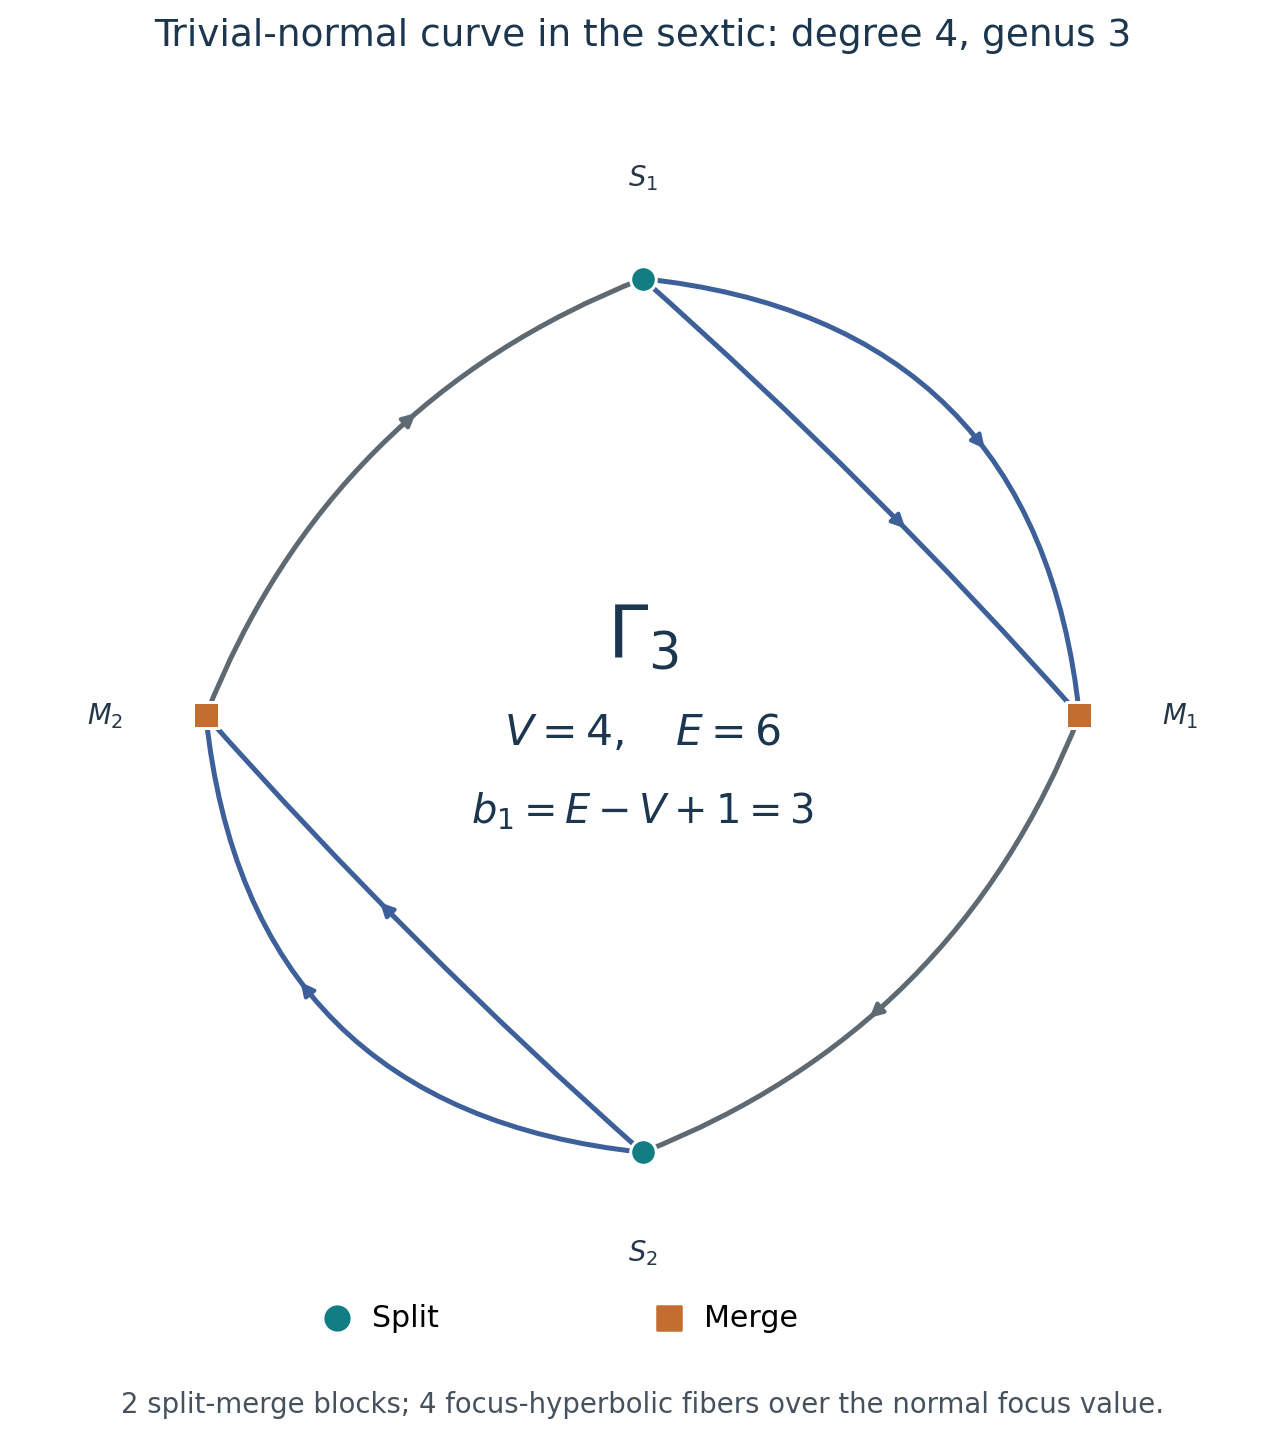
\includegraphics[width=0.73\textwidth]{trivial_normal_curve_graph.png}
 \caption{六次超曲面内の trivial-normal symplectic curve $C'$ に用いる genus-three Reeb graph。
 曲線は degree $4$、genus $3$ で、graph は4頂点・6辺・$b_1=3$を持つ。
 Actual base は $R\times\Gamma_3$ であり、normal focus value $o\in\operatorname{int}R$ と
 各 graph vertex の組の上に、Euler 数 $-1$ の whole focus--hyperbolic fiber がある。
 $\partial R$ の normal faces は残る。}
 \label{tnc:graph-figure}
\end{figure}

\begin{corollary}[残りの compact domain の Euler 数]\label{tnc:complement-euler}
上の $\mathcal U$ に対して
$\mathcal V=\overline{X_d\setminus\operatorname{int}\mathcal U}$ と置くと
\begin{equation}\label{tnc:complement-number}
 \chi(\mathcal V)
 =d(10-10d+5d^2-d^3)+(d-2)(d-5).
\end{equation}
特に六次では $\chi(\mathcal V)=-512$ である。
\end{corollary}

\begin{proof}
$\mathcal U\simeq C'\times K_c$ であり、$C'$ は closed なので
$\partial\mathcal U\simeq C'\times\partial K_c$ である。
$\partial K_c$ は corners を丸めれば closed oriented three-manifold となり、Euler 数は零である。
従って $\chi(\partial\mathcal U)=0$。
$\mathcal U$ の corners を小さい collar 内で丸める操作は、領域と complement の Euler 数を変えない。
丸めた collared boundary に沿って有限 CW 型の Euler 数の加法性を適用すると
\[
 \chi(X_d)=\chi(\mathcal U)+\chi(\mathcal V)-\chi(\partial\mathcal U)
          =-(d-2)(d-5)+\chi(\mathcal V).
\]
第\ref{bct:section}節の $\chi(X_d)$ の式を代入する。
\end{proof}

\begin{proposition}[補集合のEuler数が課すsingular fiber予算]
\label{tnc:complement-singularity-budget}
$d\ge6$ とし，系\ref{tnc:closed-block}の局所blockを
$\mathcal U\subset X_d$，そのcompact complementを$\mathcal V$とする．
次の正整数を置く：
\[
 \begin{split}
 \mathcal N_d:=-\chi(\mathcal V)
  &=d(d^3-5d^2+10d-10)-(d-2)(d-5)\\
  &=d^4-5d^3+9d^2-3d-10>0.
 \end{split}
\]
$\mathcal V$に，compact triangulable base $B_{\mathcal V}$への
proper continuous map
$f:\mathcal V\to B_{\mathcal V}$があり，
有限CW型のfiberを持つ有限stratificationに関して局所自明であると仮定する．
\emph{Euler数が非零のfiberが存在するbase pointsが有限集合
$S\subset B_{\mathcal V}$に限られる}なら，必ず
\[
 \boxed{\sum_{b\in S}\chi(f^{-1}(b))=-\mathcal N_d<0}
\]
を満たす．従ってその有限集合のfiberのEuler数がすべて
非負ということはあり得ない．
さらに，すべての$b\in S$に対して
$\chi(f^{-1}(b))=-1$なら
\[
 \boxed{|S|=\mathcal N_d}.
\]
特に$d=6$では$\mathcal N_6=512$である．
\end{proposition}
\begin{proof}
系\ref{tnc:complement-euler}によって
$\chi(\mathcal V)=-\mathcal N_d$である．
その符号は$d\ge6$で
$d(d^3-5d^2+10d-10)>(d-2)(d-5)$
から従う．実際
$d^3-5d^2+10d-10=
(d-2)(d^2-3d+4)-2$と書ける．

有限stratificationの各stratum $S_\alpha$での典型fiberを
$F_\alpha$とすると，compact支えEuler数の積公式と加法性から
\[
 \chi(\mathcal V)
   =\sum_\alpha
       \chi_c(S_\alpha)\,\chi(F_\alpha).
\]
ここで正次元stratumのcompact支えEuler数は負になり得るため，
\emph{全fiberのEuler数が非負}というだけでは
$\chi(\mathcal V)<0$に矛盾しないことに注意する．
本命題では$S$以外のfiberのEuler数が零なので，
それらのstrataの寄与は全て消え，
\[
 \chi(\mathcal V)=\sum_{b\in S}\chi(f^{-1}(b))
\]
となる．残る結論は直ちに従う．
\end{proof}

\begin{remark}[適用範囲と実際の課題]
この命題は\emph{仮に補集合の有限stratified fibrationが存在すれば}
生じる必要条件を与える．
一般のfiberには負以外のEuler数が生じてもよく，
Euler数が非零のfiberが正次元のbase stratumに並ぶ可能性もある．
従って全体のLagrangian fibrationに
$512$個の特定型fiberが必ず存在するとまでは主張しない．
現在構成済みの局所blockは$\chi(\mathcal U)=-(d-2)(d-5)$だけを担うので，
補集合の負のEuler数を説明するsingular strataを
別途設計しなければならない，という具体的な障害である．
\end{remark}

この $-512$ は、構成済みの actual domain を除いた compact complement の Euler 数である。
Complement 上の fibration はまだないため、残る singular fibers の個数とは解釈しない。

\subsection{管状補集合の整数ホモロジーと focus block との差}
\label{tnc:tubular-complement}

ここではEuler数だけでは見えない整数torsionと，
管状近傍とactual focus blockのtopologyの差を区別する．
$X_d$の三次元超曲面としての整数cohomologyについては
\cite[\S2.1]{randal-williams-hypersurface}のLefschetzおよび
Poincar\'e dualityの整理を用いる．

\begin{theorem}[閉曲線の管状補集合に現れるmeridional torsion]
\label{tnc:tubular-homology}
$d\ge6$ とし，$X_d\subset\mathbb P^4$をsmooth degree-$d$
hypersurface，$C\subset X_d$をdegree
$e=\langle\mathsf H,[C]\rangle>0$，genus $g$ の
connected closed embedded oriented surfaceとする．
そのoriented real rank-four normal disk bundleの
十分小さいclosed tubular neighborhoodを$N(C)$とし，
\[
 V_0=X_d\setminus\operatorname{int}N(C),\qquad
 b_d=d^4-5d^3+10d^2-10d+4
\]
とおく．以下は\emph{整数係数}のhomology群の同型である：
\begin{equation}\label{tnc:tubular-homology-groups}
\begin{aligned}
 H_0(V_0)&\simeq\mathbb Z,&
 H_1(V_0)&=0,&
 H_2(V_0)&\simeq\mathbb Z,\\
 H_3(V_0)&\simeq\mathbb Z^{b_d}\oplus\mathbb Z/e\mathbb Z,&
 H_4(V_0)&\simeq\mathbb Z^{2g},&
 H_k(V_0)&=0\quad(k\ge5).
\end{aligned}
\end{equation}
Normal $3$-sphere fiberのhomology classは
$H_3(V_0)$のtorsion summandを生成し，その位数は正確に$e$である．
特に定理\ref{tnc:actual-curve}のnormal-trivial curveでは
$e=d-2$であり，$d=6$なら
\[
 H_3(V_0;\mathbb Z)\simeq
       \mathbb Z^{520}\oplus\mathbb Z/4\mathbb Z,\qquad
 H_4(V_0;\mathbb Z)\simeq\mathbb Z^6,\qquad
 \chi(V_0)=-512.
\]
\end{theorem}
\begin{proof}
Lefschetzの超平面定理とPoincar\'e dualityにより
$H_1(X_d)=H_5(X_d)=0$，
$H_2(X_d)\simeq H_4(X_d)\simeq\mathbb Z$，
$H_3(X_d)\simeq\mathbb Z^{b_d}$が成り立つ．
ここで
\[
 b_d=4-\chi(X_d),\qquad
 \chi(X_d)=d(10-10d+5d^2-d^3)
\]
はChern類の計算で得られる．
Excisionとoriented codimension-fourのThom同型から
\begin{equation}\label{tnc:thom-pair}
 H_k(X_d,V_0;\mathbb Z)
 \simeq H_k(N(C),\partial N(C);\mathbb Z)
 \simeq H_{k-4}(C;\mathbb Z).
\end{equation}
対の長完全列の次数$4,3$の部分は
\[
 H_4(X_d)\xrightarrow{\;\iota_C\;}H_0(C)
 \xrightarrow{\;\partial\;}H_3(V_0)
 \longrightarrow H_3(X_d)\longrightarrow0.
\]
$H_4(X_d)$の生成元はhyperplane divisorの基本類であり，
$\iota_C$はその$C$との交点数を取る写像，
すなわち$\mathbb Z\xrightarrow{\times e}\mathbb Z$である．
従って
\[
 0\longrightarrow \mathbb Z/e\mathbb Z
 \longrightarrow H_3(V_0)
 \longrightarrow H_3(X_d)\longrightarrow0
\]
が得られる．$H_3(X_d)$は自由なので群としてsplitする．
$\partial(1)$はThom円板の境界であるnormal meridian
$S^3$を表し，その位数はちょうど$e$である．

また$H_5(X_d)=0$と
$H_5(X_d,V_0)\simeq H_1(C)=\mathbb Z^{2g}$より，
前の$\iota_C$の単射性を用いて
$H_4(V_0)\simeq H_1(C)$を得る．
同様に$H_3(X_d,V_0)=H_2(X_d,V_0)=0$より
$H_2(V_0)\simeq H_2(X_d)$，$H_1(V_0)=0$が従う．
次数$6,5$では
$H_6(X_d)\to H_6(X_d,V_0)\simeq H_2(C)$
が両者の基本類の対応による同型であることから
$H_5(V_0)=0$を得る．$V_0$は境界のあるcompact
six-manifoldなので$H_6(V_0)=0$である．
従って表示\eqref{tnc:tubular-homology-groups}を得る．
Euler数は
$2-b_d+2g=\chi(X_d)-(2-2g)$であり，六次では$-512$である．
\end{proof}

\begin{lemma}[Actual focus normal blockは円板ではない]
\label{tnc:focus-nondisk}
第\ref{fhr:section}節の
$K_c=G_c^{-1}(R)\subset\mathbb C^2$は
$H_1(K_c;\mathbb Z)$に$\mathbb Z$を直和因子として含む．
従って定理\ref{tnc:actual-curve}のclosed-curve block
$\mathcal U\simeq C'\times K_c$は，
通常の管状disk neighborhood
$C'\times D^4$とhomotopy equivalentではない．
\end{lemma}
\begin{proof}
$G_c=(P_X-P_Y,|XY-c|^2)$，
$R=[-a_*,a_*]\times[q_-,q_+]$であり
$0<q_-<c^2<q_+$である．
従って
\[
 \vartheta:K_c\longrightarrow S^1,\qquad
 (X,Y)\longmapsto\frac{XY-c}{|XY-c|}
\]
は連続である．$\sqrt{q_-}<r<c$を固定し，
$w(\theta)=c+r e^{i\theta}$と置く．
$w(\theta)\ne0$なので
\[
 X(\theta)=\sqrt{|w(\theta)|}>0,\qquad
 Y(\theta)=\frac{w(\theta)}{X(\theta)}
\]
は$K_c$内の閉曲線を定める：
$P_X-P_Y=0$，$|XY-c|^2=r^2\in(q_-,q_+)$である．
合成$\vartheta(X(\theta),Y(\theta))=e^{i\theta}$
は$S^1$のidentityだから
$\vartheta_*:H_1(K_c;\mathbb Z)\to\mathbb Z$は
split surjectiveである．
従って$H_1(K_c)$は$\mathbb Z$を直和因子に持つ．
一方$H_1(C'\times D^4)=H_1(C')$に対し
K\"unnethより$H_1(C'\times K_c)$には
$H_1(C')\oplus\mathbb Z$が直和因子として現れる．
両者の第一Betti数が異なるので同じhomotopy型ではない．
\end{proof}

\begin{proposition}[Focus block の境界torus bundleとmeridianの差]
\label{tnc:focus-boundary-homology}
$K_c$を補題\ref{fhr:focus-block}のfour-dimensional
focus blockとする．$\partial K_c$はcornersを丸めた後，
$S^1$上の$T^2$-bundleであり，fiberの一次homology上の
monodromyは適当なsymplectic integral basisで
\[
 M=\begin{pmatrix}1&1\\0&1\end{pmatrix}
\]
（基底とloopの向きによって逆または転置へ置換）である．
従って
\[
 H_1(\partial K_c;\mathbb Z)\simeq\mathbb Z^2,\quad
 H_2(\partial K_c;\mathbb Z)\simeq\mathbb Z^2,\quad
 H_3(\partial K_c;\mathbb Z)\simeq\mathbb Z.
\]
さらに$\partial K_c$の基本群は，fiberの生成元を$a,b$，
base loopを$t$とすると
\[
 \pi_1(\partial K_c)
 \simeq\langle a,b,t\mid[a,b]=1,\ 
            tat^{-1}=a,\ tbt^{-1}=ab\rangle
\]
であり，整数Heisenberg群と同型である．
この表示ではvanishing-cycle class $a=[t,b]$は
$H_1(\partial K_c;\mathbb Z)$で消えるが，
基本群では非自明である．
特に$\partial K_c$は$S^3$とhomology equivalentではなく，
closed curveに沿ったactual focus blockのnormal facesは
通常の管状disk bundleの$S^3$ facesにそのまま置換できない．
\end{proposition}
\begin{proof}
$G_c:K_c\to R$は中央$o$に一つだけ
nondegenerate focus--focus critical pointを持ち，
$\partial R$上ではregular torus fibersを持つ．
従って$\partial K_c=G_c^{-1}(\partial R)$はtorus bundleである．
一focus点の標準monodromy公式は
\cite[Section~3]{zung-focus-cf}によって
primitive unipotent transvection $M$ となる．
Wang長完全列において
\[
 H_1(T^2)=\mathbb Z^2,\quad H_2(T^2)=\mathbb Z,\qquad
 \operatorname{coker}(M-I)\simeq\mathbb Z,\quad
 \ker(M-I)\simeq\mathbb Z
\]
だから，$H_1(\partial K_c)$は
$\mathbb Z$と$\mathbb Z$のextensionであり$\mathbb Z^2$，
同じく$H_2(\partial K_c)\simeq\mathbb Z^2$．
Orientationで$H_3\simeq\mathbb Z$が従う．
またmapping torusのvan Kampen表示は
$\pi_1(T^2)\rtimes_M\mathbb Z$であり，上のrelationsになる．
$\langle a,b,t\rangle$のcommutatorは$a=[t,b]$で，
$a$は中心に属するため整数Heisenberg群の標準表示を得る．
\end{proof}

\begin{corollary}[Closed-curve focus face の整数Betti数]
\label{tnc:focus-boundary-betti}
定理\ref{tnc:actual-curve}のgenus-$g$ closed curve $C'$上の
product focus block $\mathcal U=C'\times K_c$の境界は，
cornersを丸めた後，$C'\times\partial K_c$と同相である．
その整数homologyはtorsion-freeで，
\[
 \bigl(b_0,b_1,b_2,b_3,b_4,b_5\bigr)
 =\bigl(1,\,2g+2,\,4g+3,\,4g+3,\,2g+2,\,1\bigr).
\]
さらに
\[
 \pi_1(\partial\mathcal U)
 \simeq\pi_1(C')\times H_{\mathbb Z}.
\]
特に$d=6$では$g=3$なので
\[
 (b_0,\ldots,b_5)=(1,8,15,15,8,1).
\]
\end{corollary}
\begin{proof}
$C'$はclosedであり$\mathcal U=C'\times K_c$だから
$\partial\mathcal U=C'\times\partial K_c$である．
命題\ref{tnc:focus-boundary-homology}から
$\partial K_c$の整数homologyは
$\mathbb Z,\mathbb Z^2,\mathbb Z^2,\mathbb Z$であり，
各次数でtorsionを持たない．
$H_*(C')=(\mathbb Z,\mathbb Z^{2g},\mathbb Z)$を用いる
K\"unneth formulaにより表示が得られる．
基本群はproductのvan Kampen定理による．
\end{proof}

\begin{lemma}[Normal focus domain のhomotopy型]
\label{tnc:focus-homotopy}
補題\ref{fhr:focus-block}の$K_c$は
\[
 K_c\simeq S^1\vee S^2,\qquad
 H^j(K_c;\mathbb Z)=
 \begin{cases}\mathbb Z&(j=0,1,2),\\0&(j\ge3).\end{cases}
\]
\end{lemma}
\begin{proof}
$w=XY$，$A=P_X-P_Y$とし，
$W=\{w:q_-\le|w-c|^2\le q_+\}$と書く．
$W$は$w=0$を内部に含むclosed annulusである．
$w$を固定したまま，$A$を$(1-s)A$へ変形する．
式\eqref{fhr:radii}によって，その都度
\[
 P_X(s)=\frac{\sqrt{(1-s)^2A^2+4\pi^2|w|^2}+(1-s)A}{2},
 \quad
 P_Y(s)=\frac{\sqrt{(1-s)^2A^2+4\pi^2|w|^2}-(1-s)A}{2}
\]
とし，$w\ne0$なら$X,Y$の位相を保つ．
$w=0$では非零の方の座標を$\sqrt{1-s}$倍して，
もう一方は零のままとする．これは$w=0$にも連続に延び，
$Q=|w-c|^2$を保持して$|A_s|\le a_*$なので，
$A=0$へのstrong deformation retractionを与える．

$A=0$では$|X|=|Y|=\sqrt{|w|}$であり，
$w\ne0$のfiberは$S^1$，$w=0$のfiberは一点となる．
従って
\[
 \{A=0\}\cong(W\times S^1)/(\{0\}\times S^1\text{ を潰す}).
\]
$W$を，$w=0$を固定して中央の円$\{|w-c|=c\}$
へradial deformation retractすると，右辺は
$(S^1\times S^1)/(\{*\}\times S^1)$とhomotopy equivalentである．
TorusのCW表示の一つの1-cellを潰すと，
二次cellのcommutator attaching wordは自明になるため，
$S^1\vee S^2$を得る．
\end{proof}

\begin{theorem}[Actual focus block補集合の整数homology]
\label{tnc:actual-complement-homology}
定理\ref{tnc:actual-curve}のclosed curve
$C'\subset X_d$について
$e=d-2$，$g=(d-3)(d-4)/2$，
$\mathcal U=C'\times K_c$，
$\mathcal V=\overline{X_d\setminus\operatorname{int}\mathcal U}$とおく．
$b_d=d^4-5d^3+10d^2-10d+4$とすれば
\begin{equation}\label{tnc:actual-complement-groups}
\begin{aligned}
 H_0(\mathcal V)&\simeq\mathbb Z,&
 H_1(\mathcal V)&\simeq\mathbb Z,&
 H_2(\mathcal V)&\simeq\mathbb Z^{2g+2},\\
 H_3(\mathcal V)&\simeq
  \mathbb Z^{b_d+2g+1}\oplus\mathbb Z/e\mathbb Z,&
 H_4(\mathcal V)&\simeq\mathbb Z^{2g+1},&
 H_k(\mathcal V)&=0\ (k\ge5).
\end{aligned}
\end{equation}
Torsion summandの生成元は，固定した$p\in C'$上の
focus normal face $\{p\}\times\partial K_c$の有向3-cycleである．
特に六次では
\[
 H_1(\mathcal V)=\mathbb Z,\quad
 H_2(\mathcal V)=\mathbb Z^8,\quad
 H_3(\mathcal V)=\mathbb Z^{527}\oplus\mathbb Z/4,\quad
 H_4(\mathcal V)=\mathbb Z^7,\quad
 \chi(\mathcal V)=-512.
\]
\end{theorem}
\begin{proof}
補題\ref{tnc:focus-homotopy}，K\"unnethより
$H^j(\mathcal U;\mathbb Z)$は$j=0,4$で$\mathbb Z$，
$j=1,3$で$\mathbb Z^{2g+1}$，
$j=2$で$\mathbb Z^{2g+2}$，他では零である．
Excisionと，cornersを丸めたcompact oriented
six-manifoldに対するPoincar\'e--Lefschetz双対性により
\[
 H_k(X_d,\mathcal V)\simeq
 H_k(\mathcal U,\partial\mathcal U)
 \simeq H^{6-k}(\mathcal U).
\]
この同型の下で$H_k(X_d)\to H_k(X_d,\mathcal V)$は
cohomologyの制限$H^{6-k}(X_d)\to H^{6-k}(\mathcal U)$に対応する．
$\mathcal U$は小さいnormal disk bundle
$N(C')\simeq C'$に含まれるので，次数3以上の制限は零である．
次数2ではhyperplane classの制限が
$H^2(\mathcal U)\simeq H^2(C')\oplus
(H^1(C')\otimes H^1(K_c))\oplus H^2(K_c)$
の第一因子に$e$倍で入る．

定理\ref{tnc:tubular-homology}で記した
$H_2(X_d)=H_4(X_d)=\mathbb Z$，
$H_3(X_d)=\mathbb Z^{b_d}$，
$H_1(X_d)=H_5(X_d)=0$を用いる．
次数4,3の長完全列は
\[
 0\to H^1(\mathcal U)\to H_4(\mathcal V)
 \to\mathbb Z\xrightarrow{\times e}H^2(\mathcal U)
 \to H_3(\mathcal V)\to\mathbb Z^{b_d}\to0
\]
となる．$\times e$は第一summandへの単射であり，
そのcokernelは$\mathbb Z^{2g+1}\oplus\mathbb Z/e$である．
$\mathbb Z^{b_d}$は自由なのでextensionは群としてsplitし，
$H_3,H_4$の表示を得る．
$\mathbb Z/e$の生成元は$H^2(C')$の基本classを
relative dualityで表す
$\{p\}\times[K_c,\partial K_c]$のboundary
$\{p\}\times\partial K_c$に対応する．
同様に次数3,2の制限が零なので
$H_2(\mathcal V)\simeq H^3(\mathcal U)\oplus\mathbb Z$
および$H_1(\mathcal V)\simeq H^4(\mathcal U)$が従う．
最上次数では$H_6(X_d)\to H^0(\mathcal U)$が同型で，
$H_k(\mathcal V)=0$ ($k\ge5$)を得る．
六次の数値とEuler数は式への代入である．
\end{proof}

\begin{proposition}[Focus base circuit はactual補集合の原始一次class]
\label{tnc:focus-boundary-primitive}
定理\ref{tnc:actual-complement-homology}の設定で，
normal focus map $G_c:K_c\to R$の境界
$\partial R\simeq S^1$を一周するloopを，
次のexplicit sectionで$\partial K_c$へ持ち上げる：
\[
 w=XY=c+\sqrt q>0,\quad
 X=\sqrt{P_X(A,w)/\pi}>0,\quad Y=w/X>0
 \qquad ((A,q)\in\partial R).
\]
このloopのclassを$t\in H_1(\partial K_c;\mathbb Z)$とする．
$C'$の基点$p$を固定すると
\[
 t_p=[\{p\}\times t]\in H_1(\partial\mathcal U;\mathbb Z)
\]
は$H_1(\partial\mathcal U)\to H_1(\mathcal U)$の
kernelを生成し，そのactual complementへの像は
\[
 H_1(\mathcal V;\mathbb Z)\simeq\mathbb Z
\]
の\emph{原始生成元}である（符号は向きによる）．
従って，global fillingを考える際，
normal focus base circuit を補集合側で
null-homologousにするような境界同定は不可能である．
\end{proposition}
\begin{proof}
補題\ref{tnc:focus-homotopy}の
$\vartheta:K_c\to S^1$，
$\vartheta(X,Y)=(XY-c)/|XY-c|$は
$H_1(K_c)\simeq\mathbb Z$のgeneratorを検出する．
$0<r<c$，$q_-<r^2<q_+$を固定し，
$\partial R$のface $A=a_*$上で
$w=c+r e^{i\theta}$と置く．
式\eqref{fhr:radii}によって$X>0$を選び
$Y=w/X$とすれば，このloopは
$\vartheta$の下でdegree oneとなる．
従って$H_1(\partial K_c)\to H_1(K_c)$は全射である．
命題\ref{tnc:focus-boundary-homology}により
$H_1(\partial K_c)\simeq\mathbb Z^2$だから，
そのkernelはrank oneのprimitive sublatticeである．

一方，表示したsectionは$R$全体へ延び，
$w-c=\sqrt q>0$なので$\vartheta$はsection上定数である．
従って$t$は$H_1(K_c)$で零である．
また$G_{c*}(t)$は
$H_1(\partial R)\simeq\mathbb Z$のgeneratorなので
$t$は$H_1(\partial K_c)$でprimitiveである．
ゆえに$t$がkernelを生成する．
$\partial\mathcal U=C'\times\partial K_c$と
$\mathcal U=C'\times K_c$にK\"unnethを用いると，
$H_1(\partial\mathcal U)\to H_1(\mathcal U)$は全射で，
kernelは$\mathbb Z\,t_p$である．

最後に$X_d=\mathcal U\cup\mathcal V$の
Mayer--Vietoris長完全列を用いる．
$H_1(X_d)=0$だから
\[
 H_1(\partial\mathcal U)
 \longrightarrow H_1(\mathcal U)\oplus H_1(\mathcal V)
 \longrightarrow H_1(X_d)=0
\]
の左の写像は全射である．
$H_1(\mathcal V)=\mathbb Z$は
定理\ref{tnc:actual-complement-homology}で計算済みなので，
$H_1(\mathcal U)$で零となるkernel generator $t_p$の
補集合側の像は$\pm1$でなければならない．
\end{proof}

\begin{remark}[管状補集合とactual focus補集合の比較]
\label{tnc:complement-distinction}
定理\ref{tnc:tubular-homology}の$V_0$と
定理\ref{tnc:actual-complement-homology}の$\mathcal V$は異なる．
いずれも$H_3$に位数$e=d-2$のtorsionを持つが，
\emph{自由部分と低次homologyは異なる}：
\[
 \begin{aligned}
 H_1(V_0)&=0,& H_1(\mathcal V)&\simeq\mathbb Z,\\
 \operatorname{rank}H_3(V_0)&=b_d,&
 \operatorname{rank}H_3(\mathcal V)&=b_d+2g+1 .
 \end{aligned}
\]
同じEuler数$\chi(V_0)=\chi(\mathcal V)$だけでは
これらの群は求められない．
差を支えるのは$K_c\simeq S^1\vee S^2$という局所topologyである．
第\ref{tnc:exterior-topology}節では具体的な Hopf 商を使い，
$\partial\mathcal U\to\mathcal U,\mathcal V$ の全整数 homology と
基本群の包含写像を決定する．
一方，action periods，Maslov data，coorientation と whole boundary foliation の
整合性，および relative Lagrangian filling は引き続き構成課題である．
なお$\mathbb Z/(d-2)$の補集合のtorsionと，
\cite[\S2.1]{randal-williams-hypersurface}に現れる
ambient $\pi_3(X_d)$の$\mathbb Z/d$は別の不変量である．
\end{remark}

\paragraph{閉還元面の収支との整合.}
$\nu=\mathfrak a/(d-5)$ とすれば
\[
 \operatorname{Area}(C')+\nu\chi(C')
 =(d-2)\mathfrak a-\frac{\mathfrak a}{d-5}(d-2)(d-5)=0.
\]
従って closed reduction の section が存在する場合の面積条件とも整合する。
Generic plane section $C$ の normal degree $2d$ を零へ変えたわけではなく、
degree と genus の異なる $C'$ を選んでいる。

\paragraph{大域化との距離.}
この結果は、所定の $X_d$ の actual symplectic form の下で、閉曲線全体を含む
non-elliptic focus--hyperbolic block を与える。
既存 shell の fiber relation、指定された旧 annular germs、旧48 ports の接続は保持していない。
$\partial R\times\Gamma$ の接続、残りの $X_d$ の被覆、および global base における graph cycles の処理は未構成である。
従って境界を持たない全体 fibration の存在は、引き続き未証明である。
